\documentclass[aspectratio=169,11pt,t]{beamer}
% ============================================================
%  ksa-cs-v2: ksa-cs-lecture-template.tex 스타일 + 한글, v2 덱(16:9)용.
%    - 짙은 네이비 헤드라인 (섹션 이름 + 프레임마다 점)
%    - 꽉 찬 파란 제목 막대, 둥근 그림자 블록
%    - 한글: Noto Sans CJK KR (fontspec)
%  사용:
%    \documentclass[aspectratio=169,11pt,t]{beamer}
%    \input{<..>/theme/ksa-cs-v2.tex}
%  ksa-theme.tex 의 매크로(\kb \kq, ksablue/ksared 등)도 같은 이름으로 둔다
%  -> v2 덱 본문을 거의 그대로 옮길 수 있다.
% ============================================================

\usepackage{fontspec}
\usepackage{amsmath,amssymb}
\usepackage{tikz}
\usepackage{listings}
\usepackage{graphicx}
\usepackage{booktabs}
\usepackage{varwidth}
% enumitem 은 넣지 않는다 (beamer 글머리표가 사라진다)

\defaultfontfeatures{Ligatures=TeX}
\setmainfont{Noto Sans CJK KR}
\setsansfont{Noto Sans CJK KR}
\setmonofont{Noto Sans Mono CJK KR}[Scale=0.92]
\usefonttheme{professionalfonts}

% ---------- 기본 틀 ----------
\usetheme{default}
\useinnertheme[shadow=true]{rounded}
\setbeamertemplate{navigation symbols}{}
\setbeamersize{text margin left=1em,text margin right=1em}

% ---------- 색 (템플릿 원본 값) ----------
\definecolor{navydark}{HTML}{191959}
\definecolor{navydim}{HTML}{8888B0}
\definecolor{navytitle}{HTML}{262686}
\definecolor{navyblue}{HTML}{3333B2}
\definecolor{blockbodybg}{HTML}{E9E9F3}
\definecolor{examplegreen}{HTML}{006000}
\definecolor{examplebg}{HTML}{E5EFE5}
\definecolor{alertred}{HTML}{BF0000}
\definecolor{alertbg}{HTML}{F9E5E5}
% ksa-theme.tex 와 같은 이름 (본문 호환)
\colorlet{ksablue}{navytitle}
\colorlet{ksabluedk}{navydark}
\definecolor{ksagold}{HTML}{D6CBB1}
\definecolor{ksagolddk}{HTML}{A9976B}
\colorlet{ksared}{alertred}
\definecolor{ksagray}{HTML}{5B5B5B}

\setbeamercolor{structure}{fg=navyblue}
\setbeamercolor{alerted text}{fg=alertred}
\setbeamercolor{frametitle}{bg=navytitle,fg=white}
\setbeamercolor{title}{fg=white,bg=navytitle}
\setbeamercolor{block title}{bg=navytitle,fg=white}
\setbeamercolor{block body}{bg=blockbodybg,fg=black}
\setbeamercolor{block title example}{bg=examplegreen,fg=white}
\setbeamercolor{block body example}{bg=examplebg,fg=black}
\setbeamercolor{block title alerted}{bg=alertred,fg=white}
\setbeamercolor{block body alerted}{bg=alertbg,fg=black}
\setbeamercolor{item}{fg=navyblue}
\setbeamertemplate{itemize item}[circle]
\setbeamertemplate{itemize subitem}[triangle]

% ---------- 헤드라인: miniframes (섹션 이름 + 점) ----------
\useoutertheme[subsection=false]{miniframes}
\setbeamerfont{section in head/foot}{size=\tiny}
\setbeamercolor{section in head/foot}{bg=navydark,fg=white}
\setbeamercolor{mini frame}{fg=white}
\setbeamertemplate{mini frames}[circle]

% ---------- 제목 막대: 폭 꽉 채움, 두 줄까지 ----------
\setbeamerfont{frametitle}{size=\normalsize,series=\bfseries}
\setbeamertemplate{frametitle}{%
  \nointerlineskip
  \begin{beamercolorbox}[wd=\paperwidth,ht=2.7ex,dp=1.1ex,leftskip=.3cm,rightskip=.3cm]{frametitle}%
    \usebeamerfont{frametitle}\insertframetitle
  \end{beamercolorbox}}

% ---------- 쪽 번호: 오른쪽 아래 ----------
\setbeamertemplate{footline}{%
  \hfill
  {\color{navydim}\scriptsize\insertframenumber\,/\,\inserttotalframenumber}%
  \hspace{3mm}\vspace{2mm}%
}

% ---------- 표지: 템플릿처럼 헤드라인은 그대로, 가운데 둥근 그림자 상자에 제목 한 줄 ----------
% 덱에서:  {\setbeamertemplate{footline}{}\begin{frame}[c,noframenumbering]\titlepage\end{frame}}
\setbeamercolor{title}{fg=white,bg=navyblue}
\makeatletter
\setbeamertemplate{title page}{%
  \vfill
  \centering
  \begin{minipage}{0.84\paperwidth}
  \begin{beamercolorbox}[wd=\linewidth,sep=7pt,center,rounded=true,shadow=true]{title}
    {\usebeamerfont{title}\inserttitle\par}%
    \ifx\insertsubtitle\@empty\else\vskip0.4em{\usebeamerfont{subtitle}\insertsubtitle\par}\fi
  \end{beamercolorbox}
  \end{minipage}\par\vskip1.6em
  {\usebeamerfont{author}\color{navytitle}\insertauthor\par}\vskip0.3em
  {\usebeamerfont{institute}\color{ksagray}\insertinstitute\par}
  \vfill
}
\makeatother
\setbeamerfont{title}{series=\bfseries,size=\Large}
\setbeamerfont{subtitle}{size=\normalsize}
\setbeamerfont{author}{size=\normalsize}
\setbeamerfont{institute}{size=\small}

% ksa-theme 호환: 덱이 \renewcommand{\ksacredit}{..} 를 해도 되게 (꼬리말에는 안 쓴다)
\newcommand{\ksacredit}{}

% ---------- 강조 ----------
\newcommand{\hl}[1]{\textcolor{alertred}{#1}}
\newcommand{\hlb}[1]{\textcolor{navyblue}{#1}}
\newcommand{\kb}[1]{\textbf{\color{ksablue}#1}}
\newcommand{\kq}[1]{\textbf{\color{ksared}#1}}

% ---------- 파이썬 코드 (템플릿과 같은 색) ----------
\definecolor{codekw}{HTML}{0033B3}
\definecolor{codebuiltin}{HTML}{BF0000}
\definecolor{codestr}{HTML}{067D17}
\definecolor{codecomment}{HTML}{8C8C8C}
\definecolor{codenum}{HTML}{1750EB}
\lstdefinestyle{py}{
  language=Python, basicstyle=\ttfamily\scriptsize,
  keywordstyle=\color{codekw}\bfseries, stringstyle=\color{codestr},
  commentstyle=\color{codecomment}\itshape, numberstyle=\color{codenum},
  emph={print,len,range,sum,input,int,str,float,list,dict,append,remove,sorted,abs,min,max},
  emphstyle=\color{codebuiltin}, showstringspaces=false, keepspaces=true,
  columns=fixed, basewidth=0.52em, aboveskip=1mm, belowskip=1mm, xleftmargin=2mm,
  breaklines=true
}
\lstset{style=py}

% 원본 덱 (ksa-theme): slides/v2/ml1/week10/resnet/ -- 그림은 거기 figs/ 를 그대로 쓴다
\setbeamerfont{author}{size=\normalsize}
\setbeamerfont{institute}{size=\small}
\graphicspath{{../../../v2/ml1/week10/resnet/figs/}{../../../assets/}}
\makeatletter
\newcommand{\markpage}[1]{\protected@write\@auxout{}{\string\newlabel{#1}{{\the\c@framenumber}{}}}\hypertarget{#1}{}}
\newcommand{\pref}[1]{\hyperlink{#1}{\textcolor{ksagolddk}{(p.\ref{#1})}}}
\makeatother

\renewcommand{\ksacredit}{Machine Learning and Deep Learning \,\textperiodcentered\, ResNet}
\title{ResNet 잔차 신경망 (Residual Network)}
\subtitle{입력을 건너뛰어 더하는 지름길 하나}
\author{Machine Learning and Deep Learning}
\institute{한국과학영재학교 (KSA)}
\date{}
\begin{document}
{\setbeamertemplate{footline}{}\begin{frame}[c,noframenumbering]\titlepage\end{frame}}

\section{질문}
% --- 오늘의 질문
\begin{frame}{오늘의 질문: 두 배 깊게 쌓으면 더 좋아질까?}
\vfill
\centering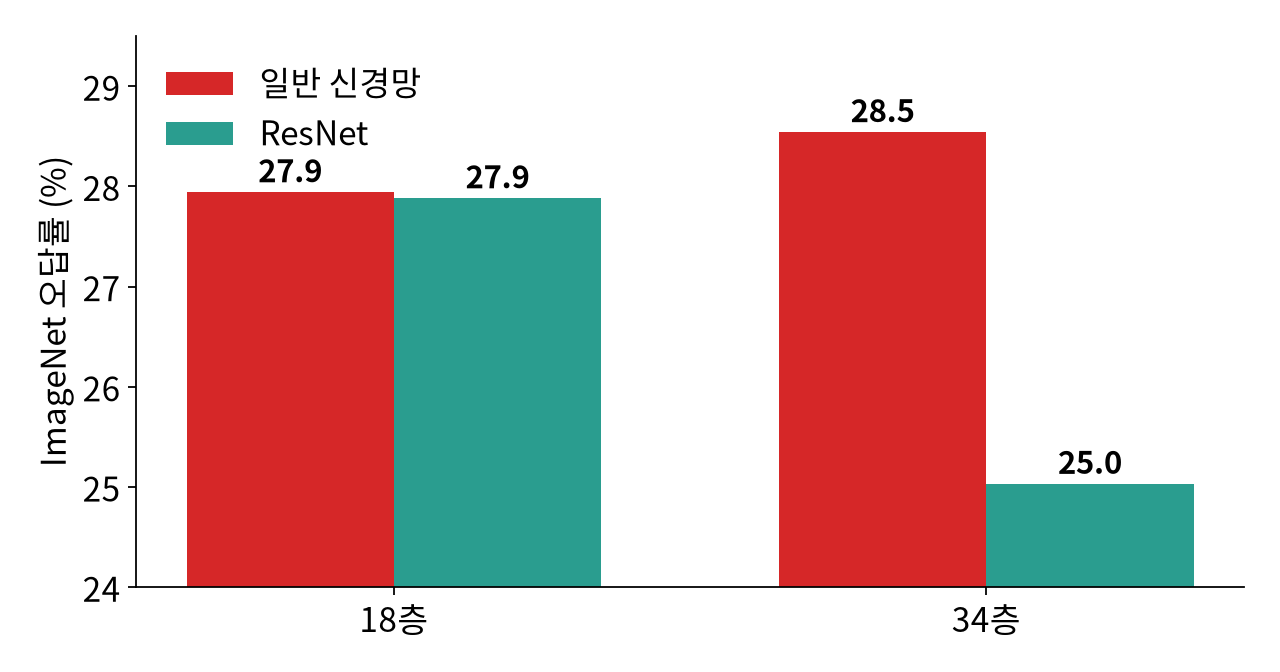
\includegraphics[width=0.52\linewidth]{rn_paper.png}\par\vskip0.2em
{\large 일반 신경망 18 $\to$ 34층: 27.9\% $\to$ \kq{28.5\%, 오히려 증가} (학습 데이터에서도)}\\[0.2em]
{\small He, Zhang, Ren, Sun (2015), ImageNet 검증 top-1 오답률}
\vfill
\note{지난 시간 CNN에서 층을 깊게 쌓을수록 더 복잡한 특징을 배운다고 했습니다. 그러면 18층을 34층으로 두 배 쌓으면 더 좋아질까요? 2015년 마이크로소프트의 허카이밍 팀이 실험해 보니, 일반 신경망은 이미지넷 오답률이 27.9퍼센트에서 28.5퍼센트로 오히려 늘었습니다. 놀라운 점은 학습 데이터에서도 더 못했다는 겁니다. 과대적합이라면 학습 데이터에서는 더 잘해야 하는데, 그게 아니라 깊은 신경망이 학습 자체를 제대로 못 한 겁니다. 같은 팀의 해결책, 오른쪽 초록 막대 ResNet은 34층에서 25.0퍼센트로 줄었습니다.}
\end{frame}

\section{잔차 연결}
% --- 이상한 점
\begin{frame}{이상하다: 깊은 쪽이 최소한 같아야 한다}
\vfill
\centering
{\large 18층 신경망에 층 16개를 더 붙이는데, 그 16개가 \textbf{입력을 그대로 내보내기만} 하면}\\[0.6em]
{\Large 34층 = 18층과 \kb{정확히 같은} 성능}\\[1.0em]
{\large 34층이 더 나쁠 이유가 없다 \quad 그런데 ``그대로 내보내기'' 조차 \kq{학습하기 어렵다}}\\[0.6em]
{\small 여러 층을 거쳐 $\mathbf{h} = \mathbf{x}$ 를 만들기는 까다롭다 (기울기 소실과도 얽힘)}
\vfill
\note{생각해 보면 이상합니다. 18층 신경망 뒤에 층 16개를 더 붙여 34층을 만든다고 해 봅시다. 붙인 16개 층이 입력을 그대로 내보내기만 해도 34층은 18층과 정확히 같은 성능을 냅니다. 그러니 34층이 더 나쁠 이유가 없습니다. 그런데 실제로는 이 그대로 내보내기조차 경사하강법으로 찾기 어렵습니다. 가중치 행렬과 ReLU를 여러 번 거치면서 출력이 입력과 똑같이 나오게 맞추는 것은 생각보다 까다롭고, 지난주의 기울기 소실 문제와도 얽혀 있습니다.}
\end{frame}

% --- 잔차 블록
\begin{frame}{해결: 입력을 건너뛰어 더한다}
\markpage{block}
\vfill
\centering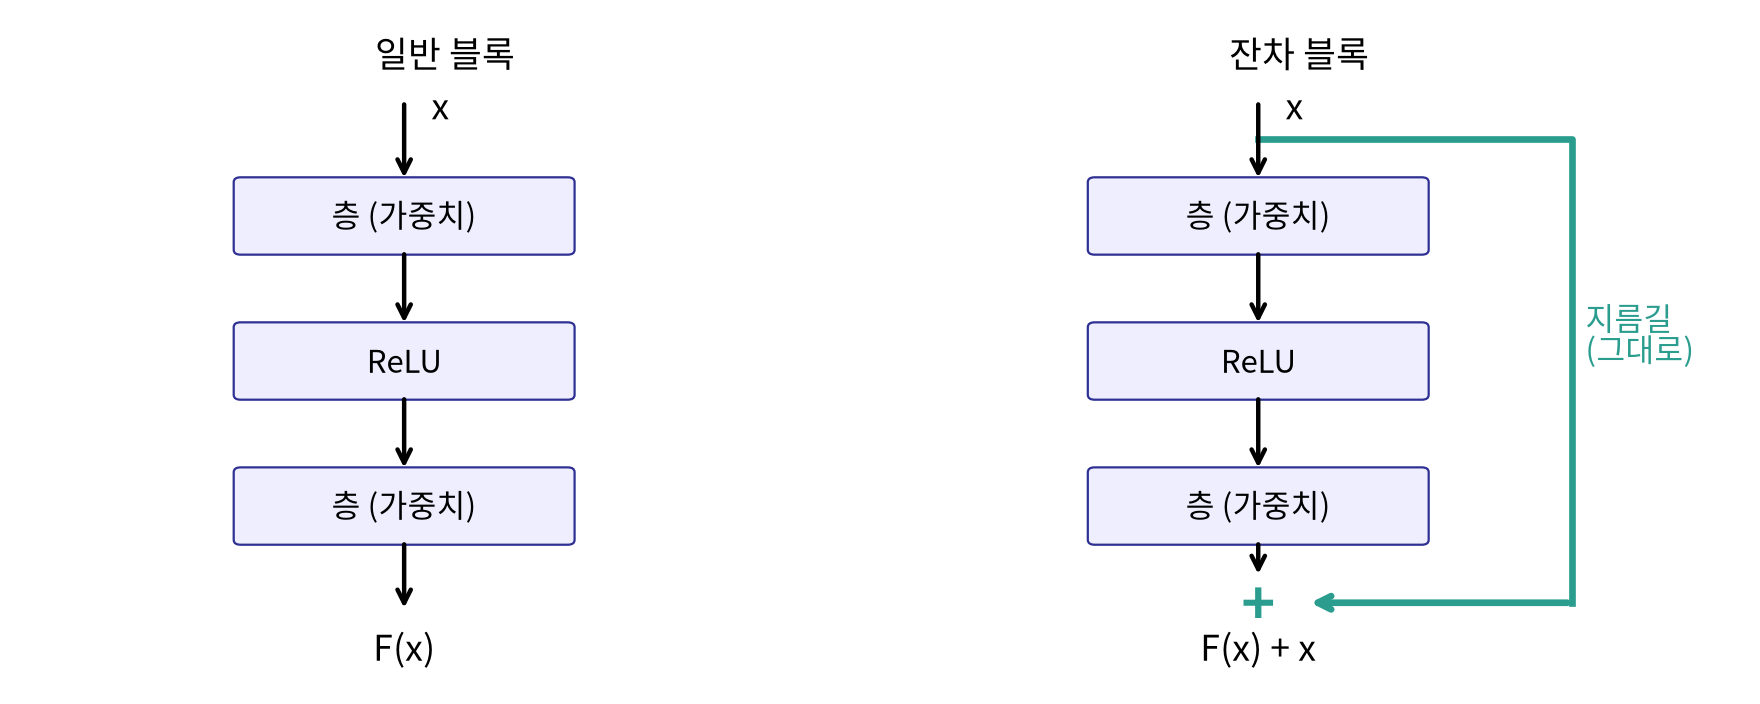
\includegraphics[width=0.68\linewidth]{rn_block.png}\par\vskip0.2em
{\LARGE\[ \mathbf{y} = F(\mathbf{x}) + \mathbf{x} \]}
{\small 지름길 (skip connection, shortcut) \quad 가중치가 없다, 그냥 더하기}
\vfill
\note{해결책은 지름길 하나입니다. 층 두 개를 거친 결과 F(x)에 입력 x를 그대로 더합니다. 출력은 F(x) 더하기 x입니다. 이 지름길에는 가중치가 없습니다. 입력을 두 층 건너뛰어 출력에 더할 뿐입니다. 이런 블록을 잔차 블록이라고 하고, 이 블록을 쌓은 신경망이 ResNet, 잔차 신경망입니다.}
\end{frame}

% --- 잔차만 배운다
\begin{frame}{층은 \textbf{바뀔 부분 (잔차)} 만 배운다}
\vfill
\centering
{\Large 원하는 출력이 $H(\mathbf{x})$ 라면 \quad 층이 배울 것은 \quad $F(\mathbf{x}) = H(\mathbf{x}) - \mathbf{x}$}\\[1.0em]
\renewcommand{\arraystretch}{1.5}
{\large\begin{tabular}{ll}
할 일이 없으면 & $F = 0$ $\to$ 입력이 \kb{그대로} 통과\\
조금 고칠 일이면 & 작은 수정만 배운다\\
역전파 & $\partial \mathbf{y}/\partial \mathbf{x} = \partial F/\partial \mathbf{x} + 1$ $\to$ 기울기가 \kb{줄지 않고} 전달
\end{tabular}}
\vfill
\note{지름길이 왜 도움이 될까요? 블록이 원래 내야 할 출력을 H(x)라고 하면, 지름길이 x를 이미 더해 주니 층들은 H(x) 빼기 x, 즉 입력에서 바뀌어야 할 부분만 배우면 됩니다. 이것을 잔차라고 합니다. 할 일이 없는 블록은 F가 0만 내면 되고, 가중치를 0 근처로 두는 건 쉽습니다. 입력이 그대로 통과합니다. 역전파 쪽에서 보면, y를 x로 미분하면 F의 미분 더하기 1입니다. 이 1 덕분에 기울기가 층마다 곱해져 사라지지 않고 지름길을 따라 앞 층까지 그대로 전달됩니다.}
\end{frame}

\section{결과}
% --- 결과
\begin{frame}{결과}
\vfill
\centering
\renewcommand{\arraystretch}{1.5}
{\Large\begin{tabular}{lcc}
ImageNet top-1 오답률 & 18층 & 34층\\\hline
일반 신경망 & 27.9\% & \kq{28.5\%}\\
ResNet & 27.9\% & \kb{25.0\%}
\end{tabular}}\vskip0.8em
{\large \textbf{152층}까지 쌓아 ILSVRC 2015 1위 (상위 5개 오답률 \kb{3.57\%}, 앙상블)}\\[0.4em]
{\small He, Zhang, Ren, Sun (2015) arXiv:1512.03385, Table 2 \quad 인용 수가 가장 많은 논문 중 하나}
\vfill
\note{결과입니다. 18층에서는 두 신경망이 27.9퍼센트로 거의 같습니다. 34층으로 깊게 하면 일반 신경망은 28.5퍼센트로 나빠지지만, ResNet은 25.0퍼센트로 좋아집니다. 이제 깊게 쌓을수록 좋아지는 겁니다. 이 팀은 152층까지 쌓아 2015년 이미지넷 대회에서 상위 5개 오답률 3.57퍼센트로 1위를 했습니다. 이 논문은 과학 전체를 통틀어 가장 많이 인용된 논문 중 하나입니다.}
\end{frame}

% --- 우리 실험
\begin{frame}{우리 실험: 손글씨 1만 장, 깊이만 바꿨다}
\markpage{ours}
\vfill
\centering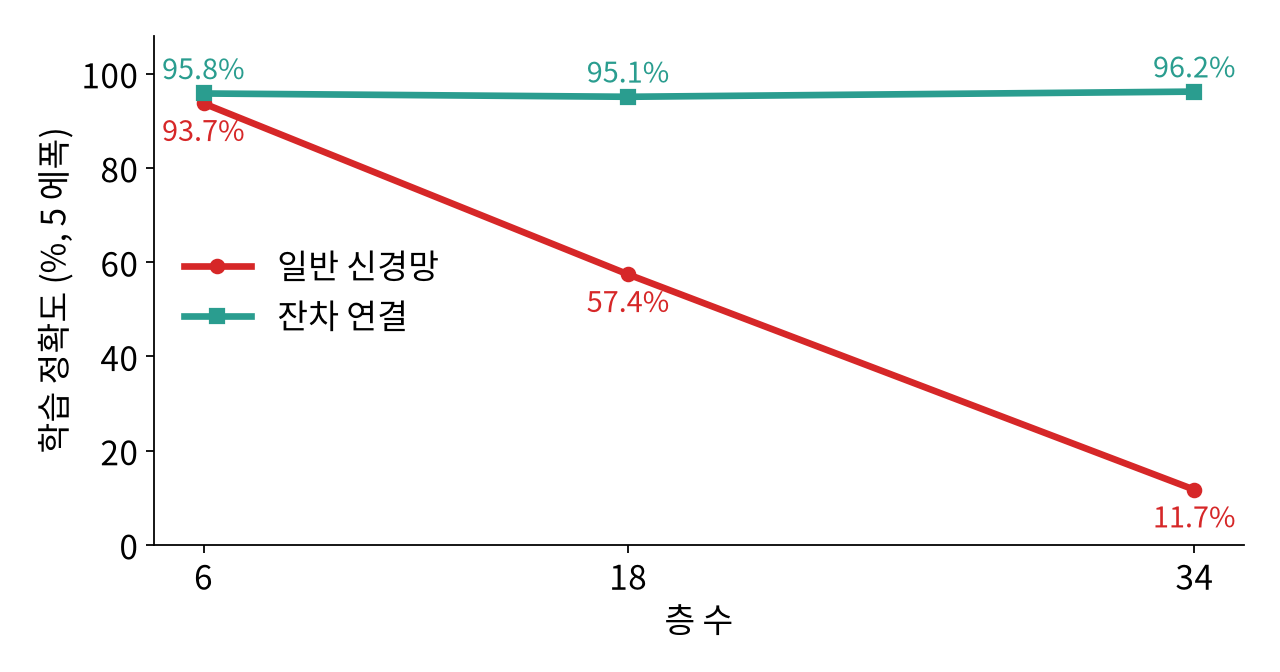
\includegraphics[width=0.56\linewidth]{rn_ours.png}\par\vskip0.2em
{\large 34층: 일반 \kq{11.7\%} (못 배움) \quad 잔차 \kb{96.2\%} \quad (학습 정확도, 5 에폭)}\\[0.2em]
{\small 블록 = 층 2개 (폭 64) \quad 블록 2 · 8 · 16개 = 층 6 · 18 · 34개 \quad Adam, 같은 조건}
\vfill
\note{우리도 직접 실험해 봤습니다. 손글씨 숫자 1만 장으로, 층 두 개짜리 블록을 2개, 8개, 16개 쌓았습니다. 층 수로는 6, 18, 34층입니다. 일반 신경망은 6층에서 학습 정확도 93.7퍼센트지만, 18층에서 57.4퍼센트, 34층에서는 11.7퍼센트로 아예 배우지 못했습니다. 지름길 하나만 넣은 잔차 신경망은 6층, 18층, 34층 모두 95퍼센트가 넘습니다. 깊이를 늘려도 학습이 무너지지 않습니다.}
\end{frame}

\section{쓸 때}
% --- 크기가 다를 때
\begin{frame}{더하려면 크기가 같아야 한다}
\vfill
\centering
{\large CNN 에서는 중간에 채널 수가 늘고 (64 $\to$ 128) 크기가 줄어든다 (보폭 2)}\\[0.6em]
{\Large\[ \mathbf{y} = F(\mathbf{x}) + W_s\,\mathbf{x} \]}\vskip0.2em
{\large 그때만 지름길에 \textbf{1 × 1 합성곱} $W_s$ 를 넣어 크기를 맞춘다 \quad 나머지 지름길은 그냥 더하기}\\[0.8em]
{\small ResNet 블록 = 합성곱 $\to$ BatchNorm $\to$ ReLU $\to$ 합성곱 $\to$ BatchNorm $\to$ (+ 지름길) $\to$ ReLU}
\vfill
\note{하나 짚고 넘어갈 점은, 더하려면 F(x)와 x의 크기가 같아야 한다는 겁니다. CNN에서는 중간에 채널 수가 64에서 128로 늘거나 보폭 2로 크기가 줄어드는 곳이 있습니다. 그런 곳에서만 지름길에 1 곱하기 1 합성곱을 넣어 채널과 크기를 맞춥니다. 나머지 대부분의 지름길은 그냥 더하기입니다. 실제 ResNet 블록은 합성곱, 지난주의 BatchNorm, ReLU, 합성곱, BatchNorm을 거친 뒤 지름길을 더하고 ReLU를 씌웁니다.}
\end{frame}

% --- 지금
\begin{frame}{지름길은 지금 어디에나 있다}
\vfill
\centering
\renewcommand{\arraystretch}{1.5}
{\large\begin{tabular}{ll}
\textbf{이미지} & ResNet-50 은 지금도 이미지 모델의 기준선\\
\textbf{트랜스포머} (12주차) & 모든 층이 $\mathbf{x} + \text{Attention}(\mathbf{x})$, \; $\mathbf{x} + \text{FFN}(\mathbf{x})$\\
\textbf{GPT · BERT} & 수십 $\sim$ 백 층 이상을 쌓을 수 있는 이유 중 하나
\end{tabular}}\vskip0.8em
{\large ``바꿀 부분만 배우고, 나머지는 그대로 흘려보낸다''}
\vfill
\note{이 지름길은 지금 딥러닝 어디에나 있습니다. ResNet-50은 지금도 이미지 모델의 기준선으로 쓰입니다. 12주차에 배울 트랜스포머는 모든 층이 x 더하기 어텐션, x 더하기 FFN 모양입니다. GPT나 BERT가 수십에서 백 층 넘게 쌓을 수 있는 이유 중 하나가 이 지름길입니다. 바꿀 부분만 배우고 나머지는 그대로 흘려보낸다는 생각이 딥러닝의 기본이 되었습니다.}
\end{frame}

\section{연습}
% --- 문제풀이
\begin{frame}{문제풀이}
\vfill
\begin{enumerate}
\item 잔차 블록에서 $\mathbf{x} = (1, 2)$, $F(\mathbf{x}) = (0.1, -0.3)$ 이면 출력은? 블록이 아무것도 안 바꾸려면 $F$ 는?\vskip0.8em
\item 일반 신경망 50층의 학습 정확도가 20층보다 낮다. 과대적합인가? 이유는?\vskip0.8em
\item $y = F(x) + x$ 에서 $\partial F / \partial x = 0.01$ 이면 $\partial y / \partial x$ 는? 지름길이 없으면?\vskip0.8em
\item 입력 채널 64, 출력 채널 128 인 블록의 지름길에 쓰는 1 × 1 합성곱의 가중치 수는? (편향 없음)
\end{enumerate}
\vfill
\note{1번 답. (1.1, 1.7)이고, 아무것도 안 바꾸려면 F가 (0, 0)이면 됩니다. 2번 답. 과대적합이 아닙니다. 과대적합이면 학습 데이터에서는 더 잘해야 하는데 더 못하니, 깊어서 최적화가 어려운 문제입니다. 3번 답. 1.01이고, 지름길이 없으면 0.01입니다. 층마다 곱해지면 차이가 엄청나게 커집니다. 4번 답. 64 곱하기 128, 8192개입니다.}
\end{frame}

% --- 실습
\begin{frame}{실습}
\vfill
\centering\begin{tabular}{rl}
\large 1 & 잔차 블록 직접 만들기 (\texttt{nn.Module}, \texttt{F(x) + x})\\[0.5em]
\large 2 & 손글씨 1만 장: 일반 vs 잔차, 6 · 18 · 34층 $\to$ 11.7\% vs 96.2\% 재현\\[0.5em]
\large 3 & 층별 기울기 크기 비교 + torchvision \texttt{resnet18} 구조 들여다보기
\end{tabular}\vskip1em
MNIST (torchvision) \\[0.4em]\href{https://colab.research.google.com/github/SuminHan/book-ml/blob/main/slides/v2/ml1/week10/resnet/lab/resnet.ipynb}{\textcolor{ksagolddk}{▶ Colab에서 실습 노트북 열기}}
\vfill
\note{실습은 세 부분입니다. 첫째, PyTorch로 잔차 블록을 직접 만듭니다. forward에서 F(x) 더하기 x를 돌려주면 됩니다. 둘째, 손글씨 1만 장으로 일반 신경망과 잔차 신경망을 6, 18, 34층으로 쌓아 오늘의 결과를 재현합니다. 셋째, 두 신경망의 층별 기울기 크기를 비교하고, torchvision에 들어 있는 실제 resnet18의 구조를 들여다봅니다.}
\end{frame}

\section{정리}
% --- 정리
\begin{frame}{정리}
\vfill
\centering\large\begin{tabular}{l}
깊게 쌓은 일반 신경망은 \textbf{학습 데이터에서도} 더 못한다 (18 $\to$ 34층: 27.9 $\to$ 28.5\%)\\[0.5em]
\textbf{잔차 블록} $\mathbf{y} = F(\mathbf{x}) + \mathbf{x}$ \quad 층은 바뀔 부분만, 할 일 없으면 0\\[0.5em]
기울기가 지름길로 그대로 전달 ($+1$) \quad 34층 25.0\%, 152층으로 2015 대회 1위\\[0.5em]
우리 실험 34층: 일반 11.7\% vs 잔차 96.2\% \quad 트랜스포머의 모든 층에도
\end{tabular}
\vfill
\note{정리합니다. 일반 신경망을 깊게 쌓으면 과대적합이 아니라 학습 데이터에서조차 더 못하게 됩니다. ResNet은 입력을 건너뛰어 출력에 더하는 지름길 하나로 이 문제를 풀었습니다. 층들은 바뀔 부분, 잔차만 배우면 되고, 할 일이 없으면 0만 내면 됩니다. 역전파에서는 기울기가 지름길로 그대로 전달됩니다. 그 결과 34층에서 25.0퍼센트로 좋아졌고, 152층까지 쌓아 2015년 대회에서 1위를 했습니다. 우리 실험에서도 34층 일반 신경망은 11.7퍼센트, 잔차 신경망은 96.2퍼센트였습니다. 이 지름길은 지금 트랜스포머의 모든 층에도 들어 있습니다.}
\end{frame}
\end{document}
